\chapter{Experiments} % Experimental Study of Watershed Weighting Strategies}
\label{Chapter5}
The majority of our experiments focuses on weighting the watershed locations. That corresponds to the \textbf{Structured voting (SV)} stage of the pipeline that we propose for the task of going from edges to contours: SE-SV-UCM.

\textbf{Dataset:} For the evaluation of our segmentation results we work on the Berkeley Segmentation Data Set (BSDS500)~\cite{Arbelaez11}. Since its introduction in 2001, it has by now become a standard dataset for both the task of edge detection as well as that of image segmentation.

\textbf{Two evaluation metrics - BPR and VPR:} We look at two Precision-recall metrics. One is the Boundary Precision-Recall (BPR)~\cite{Arbelaez11} which is a boundary-based metric and emphasises the correct placement of image edges. In case of segmentation, BPR is a good indicator of the localisation of the region boundaries. A difference in the score of a single region boundary pixel should not greatly affect the edge detector output. Therefore, it correctly has only a small impact on the BPR metric. For the task of image segmentation however, a change in a single pixel could result in merging neighbouring regions. In the hierarchical image segmentation framework, that means multiple levels of the segmentations hierarchy would change. So a rigorous image segmentation benchmark metric should not be oblivious to such changes. To address this issue, the other metric that we report is the Volume Precision-Recall (VPR)~\cite{Galasso13} introduced to evaluate the accuracy of video segmentation algorithms. For images (or video still frames) the metric is a region-based metric, measuring the size of the regions and the overlap between the ground truth segmentation regions and the algorithm under test.

\textbf{Watershed weighting strategy:} The Structured voting requires a choice of a watershed weighting strategy. The purpose of the weighting is associating a score with each of the watershed locations pixels. That score must faithfully reflect the strength of the underlying boundary. So we want to evaluate how good a boundary evidence the most likely segmentation determined by the structured forests presents. The first aspect of it is making the structured forest patch and the watershed locations patch comparable. The watershed patch is an oversegmentation, and in this sense, contains much more information, not exclusively about the location of the boundary that we would like to evaluate. So we strive to simplify the watershed patch, keeping only important information about it - the shape of the boundary under consideration, or the constitution of the segmentation in the patch. Such a simplification in the context of our algorithm we call ``watershed patch transformation''. The second particular to a watershed weighting strategy is the choice of scoring function. We view the task as a segmentation benchmark problem, where one of the patches is the ground truth segmentation, and the other - the segmentation under test. We analyse and apply a selection of boundary- and region- based metrics.

\textbf{Oracle} To evaluate the correctness of our weighting strategies, we've implemented an oracle for our pipeline. The question we wanted to answer is ``how well could we perform segmentation in the presence of perfect information?'' Our Structured voting lends itself easily to such an experiment using the ground truth segmentation. When scoring a given pixel on the watershed regions boundary, we use a ground truth segmentation patch, rather than the most likely segmentation learnt by the structured forest. The second patch, as in the regular experiments, comes from the watershed locations image, taken for the same pixel location.

\section{Evaluation}
\subsection{Dataset}
The Berkeley Segmentation Data Set (BSDS), introduced in~\cite{Martin01}, is a large dataset of natural images that have been manually segmented by multiple participants. It, therefore, provides the ground truth label for each pixel as being on- or off-boundary. Initially the dataset featured 300 images (BSDS300). It was later extended - in BSDS500~\cite{Arbelaez11} the original 300 images are used for training (200) and validation (100), and 200 new human-annotated images are added for testing. Again, each image is segmented by different subjects.

\begin{figure}[ht!]
 \centering
 \subfigure[Input image]{%
 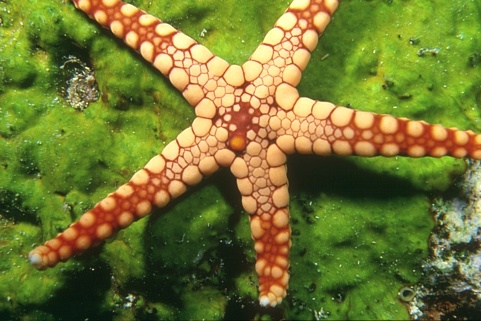
\includegraphics[width=0.3\textwidth]{images/examples/starfish/starfish.png}
 }
 \subfigure[Segmentation by subject 1]{%
 
\includegraphics[width=0.3\textwidth]{images/examples/starfish/starfish_segm_coarse.png}
 }
 \subfigure[Boundaries by subject 1]{%
 
\includegraphics[width=0.3\textwidth,frame]{images/examples/starfish/starfish_bdry_coarse.png}
 }
 \subfigure[Segmentation subject 2]{%
 
\includegraphics[width=0.3\textwidth]{images/examples/starfish/starfish_segm_detail.png}
 }
 \subfigure[Boundaries subject 2]{%
 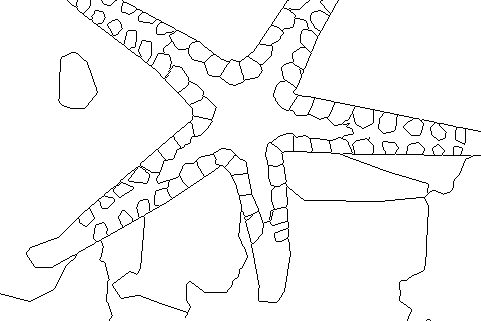
\includegraphics[width=0.3\textwidth,frame]{images/examples/starfish/starfish_bdry_detail.png}
 }
 \caption{Image from the validation subset of~\cite{BSDS500resources} and two of its annotations.}
\end{figure}

\subsection{Metrics}
\section{Weighting strategies} % Exploration of the Space of Weighting Strategies}
\section{Oracle} %  - Experiments with Ground Truth}
\subsection{Oracle definition} % description}
\subsection{Ranking of oracles}
% \subsubsection{Confirms Correct Weighting Strategies}
% \subsubsection{Failure Cases}
